% !TeX program = xelatex
\documentclass{llncs}

\usepackage{fontspec}
\setmainfont{Liberation Serif}
\setsansfont{Liberation Sans}
\usepackage{graphicx}
\usepackage{amsmath}
\usepackage{amssymb}
\usepackage{array}
\usepackage{booktabs}
\usepackage{multirow}
\usepackage{tikz}
\usepackage{pgfplots}
\usepackage{pgf-pie}
\pgfplotsset{compat=1.17}
\usetikzlibrary{arrows.meta, positioning, shapes.geometric}

\begin{document}

\title{CropState-Vision: Reliable Six-Stage Rice Growth
Classification and Confidence-Aware Stage-Gated Retrieval from Field Images}

\author{Lê Bảo Nhi \and Phan Nguyễn Quốc Minh \and Lê Khánh Nhi}

\institute{FPT University, Da Nang, Viet Nam\\
\email{lebaonhi0805@gmail.com, minhpnq1807@gmail.com, nhilekhanh29@gmail.com}}

\maketitle

\begin{abstract}
Agricultural recommendations depend on crop development, so a decision-support system must first recognize the growth stage and then retrieve stage-appropriate guidance. This paper presents CropState-Vision, which classifies field images into six BBCH-derived rice macro-stages and uses the full stage distribution to gate evidence retrieval. Beyond raw accuracy, our emphasis is evaluation reliability and retrieval safety. On a 2{,}900-image benchmark derived from RiceSEG, we first audit the splits for near-duplicate leakage and find them leak-free at every reasonable perceptual-hash threshold, so the reported scores are not inflated by memorization. Using a fixed-split, three-seed protocol we compare three training objectives for a ResNet-18 classifier: cross-entropy reaches 0.807 accuracy, an ordinal-aware loss leaves overall accuracy unchanged but stabilizes recall on the safety-critical reproductive stage (identical across seeds, $\sigma=0.000$ versus $0.071$ for cross-entropy), and a focal loss degrades calibration and is kept only as a negative ablation. We recast confidence handling as selective prediction: abstaining on the least-confident ${\sim}37\%$ of cases halves the error rate ($0.205\to0.097$). Finally, on 420 automatically-derived retrieval scenarios, confidence-adaptive soft gating matches the strongest baseline in ranking quality while reducing stage-incompatible retrievals about threefold; a stratified analysis shows the advantage holds when the prediction is correct or off by one adjacent stage but that hard filtering is safer under rare non-adjacent errors. Because these retrieval relevance labels are auto-derived from stage-compatibility rather than domain-reviewed, the retrieval results are reported as a preliminary automated evaluation, not expert-judged effectiveness. CropState-Vision claims no new architecture or dataset; the contribution is a reliable, safety-oriented evaluation of the full classification-to-retrieval pipeline.

\keywords{rice growth stage \and BBCH \and image classification \and ordinal loss \and calibration \and selective prediction \and stage-aware retrieval \and data leakage}
\end{abstract}

\section{Introduction}

Agricultural management follows the crop, not the calendar. Water management, nutrient application, disease surveillance, and harvest preparation all differ across establishment, tillering, reproductive development, grain filling, and ripening, so a digital advisor needs to know which stage a field is in before it can retrieve safe, timely guidance.

Field images are a natural input, because phenological development shows up visually through leaf development, tiller formation, stem elongation, panicle emergence, grain formation, and ripening. In practice, stage recognition is hardest exactly where it matters: near stage boundaries, and under everyday variation in viewpoint, lighting, plant density, background, and camera distance. A model can also be confidently wrong, which is a particular risk for a class with few training examples. Converting an uncertain visual prediction into a single stage label and applying a hard metadata filter can then amplify the error by discarding all evidence associated with the true stage.

CropState-Vision represents crop development as a distribution over stages rather than a single static label. Image classification supplies the visual evidence; the distribution becomes a stage belief that controls how strongly the retriever favors stage-compatible evidence. When the prediction is concentrated and calibrated, stage compatibility receives more weight; when it is diffuse, the system relaxes stage conditioning to preserve recall. After an image is uploaded, the system retrieves evidence for a fixed set of care topics rather than answering free-form questions.

This paper asks two questions. First, how reliably can six rice macro-stages be recognized from field images, once the benchmark is audited for leakage and the classifier is evaluated across seeds rather than on a single lucky run? Second, is confidence-aware soft gating more robust than top-1 hard filtering when the image-based prediction is uncertain or wrong? The contributions are:
\begin{enumerate}
    \item a leak-free benchmark audit that sweeps a perceptual-hash near-duplicate detector over 2{,}900 images and confirms zero cross-split leaking pairs at any reasonable threshold, a prerequisite for trusting every downstream number;
    \item a reliable stage-classification evaluation using a fixed-split, multi-seed protocol that separates initialization variance from split variance, showing that an ordinal-aware loss stabilizes reproductive-stage recall without changing accuracy, plus a selective-prediction analysis showing the error rate halves when the model abstains on its least-confident cases;
    \item a confidence-aware soft-gating retriever that uses the full visual distribution instead of only the top-1 stage, and an end-to-end evaluation over 420 auto-derived scenarios showing it matches the strongest baseline in ranking quality while cutting stage-incompatible retrievals about threefold;
    \item an explicit, honest account of the limitations---an underpowered reproductive subset, auto-derived rather than expert-reviewed relevance labels, and simulated temporal fusion---that bound how far these results can be pushed.
\end{enumerate}

\section{Related Work}

\subsection{Phenological Growth Stages and BBCH}

The BBCH scale gives standardized numerical descriptions of observable plant development \cite{meier2001bbch,lancashire1991uniform}: the first digit marks a principal stage, the second a more detailed sub-stage. We group fine-grained rice codes into six macro-stages for image classification; this grouping is an experimental convenience and is not meant to replace the BBCH standard itself. A systematic review of deep learning in plant phenology found that most existing studies still target only a handful of coarse stages and rarely report calibration or ordinal error structure \cite{katal2022deep}---a gap the evaluation protocol here is designed to address.

\subsection{Image-Based Rice Growth-Stage Recognition}

Machine-learning methods have already been used to estimate rice development from field or aerial imagery \cite{tan2022machine}. Detection-based work such as RiceRes2Net pairs a Res2Net backbone with a feature pyramid network to localize rice panicles and recognize growth stage at the same time \cite{tan2023ricepanicle}, and lighter YOLO variants of the same idea have since shipped as smartphone applications \cite{zheng2025android}. These systems target panicle-level detection across three reproductive sub-stages; CropState-Vision instead classifies whole images across the full vegetative-to-ripening range. Across this literature, reported performance depends heavily on how stages are defined, how images were captured, sample size, and how the train/test split was constructed---a model that looks accurate on a random split can still fail on a new field or season if it picked up background or acquisition cues rather than plant morphology, which is why we audit for leakage explicitly \cite{kapoor2023leakage}.

\subsection{Transfer Learning and Confidence}

ResNet and EfficientNet are now standard pretrained backbones for image classification \cite{he2016deep,tan2019efficientnet}, built on the earlier line of AlexNet \cite{krizhevsky2012alexnet}, VGG \cite{simonyan2015vgg}, and batch normalization \cite{ioffe2015batchnorm}. Vision Transformers offer a patch-based alternative \cite{dosovitskiy2021vit}, though their appetite for data makes them a harder fit for a small collection than an ImageNet-pretrained CNN \cite{deng2009imagenet,pan2010survey}. Accuracy alone is not the whole story: a downstream system needs to know when to trust a prediction, and calibration methods such as temperature scaling exist precisely to check whether softmax confidence tracks empirical correctness \cite{guo2017calibration}, building on earlier binning-based estimators of calibration error \cite{naeini2015calibration}.

\subsection{Class Imbalance, Ordinal Structure, and Reliable Evaluation}

The reproductive and grain-filling stages in this collection are severely under-represented, a familiar problem in image classification; focal loss \cite{lin2017focal} and data augmentation \cite{shorten2019survey} are two standard mitigations. The six macro-stages are also ordered rather than nominal, and the ordinal-regression literature is clear that treating ordered labels as if they had no order throws away useful structure \cite{gutierrez2016ordinal}---hence our use of an ordinal-aware loss and MASD alongside accuracy. The statistical protocol follows established practice: non-parametric bootstrap confidence intervals \cite{efron1993bootstrap}, Holm-corrected paired significance tests \cite{holm1979sequential}, and McNemar's test for paired binary outcomes \cite{mcnemar1947note}.

\subsection{Stage-Aware and Hybrid Retrieval}

Retrieval-augmented generation grounds model outputs in external evidence \cite{lewis2020rag}. Sparse retrieval such as BM25 captures lexical correspondence \cite{robertson2009bm25}, dense retrieval captures semantic similarity \cite{karpukhin2020dpr}, and Reciprocal Rank Fusion (RRF) combines ranked lists without directly comparing heterogeneous raw scores \cite{cormack2009rrf}. CropState-Vision uses BM25 and dense retrieval for candidate generation, then applies confidence-aware stage re-ranking. Table~\ref{tab:positioning} situates the vision side relative to the closest prior rice studies: they cover a narrower slice of the growth cycle or report accuracy-family metrics only, whereas CropState-Vision combines full-cycle stage coverage with calibration, an ordinal metric, significance testing, and a leakage audit.

\begin{table}[t]
\centering
\caption{How CropState-Vision's scope and evaluation protocol compare to the closest prior rice growth-stage studies.}
\label{tab:positioning}
\small
\begin{tabular}{p{0.24\textwidth}p{0.24\textwidth}>{\centering\arraybackslash}p{0.1\textwidth}>{\centering\arraybackslash}p{0.11\textwidth}p{0.19\textwidth}}
\toprule
\textbf{Study} & \textbf{Stage coverage} & \textbf{Calib.} & \textbf{Ordinal} & \textbf{Sig. testing} \\
\midrule
Seedling HOG-SVM / EfficientNet \cite{tan2022machine} & 3 seedling sub-stages & -- & -- & -- \\
RiceRes2Net \cite{tan2023ricepanicle} & 3 reproductive sub-stages (panicle-level) & -- & -- & -- \\
Smartphone YOLO app \cite{zheng2025android} & 3 reproductive sub-stages (panicle-level) & -- & -- & -- \\
\textbf{CropState-Vision (this work)} & \textbf{6 macro-stages, establishment--ripening} & \textbf{ECE, Brier} & \textbf{MASD} & \textbf{Bootstrap CI, McNemar} \\
\bottomrule
\end{tabular}
\end{table}

\section{Task Formulation}

\subsection{Research Questions and Hypotheses}

Table~\ref{tab:rq} lists the research questions and the hypothesis attached to each.

\begin{table}[t]
\centering
\caption{Research questions and hypotheses.}
\label{tab:rq}
\small
\begin{tabular}{p{0.06\textwidth}p{0.46\textwidth}p{0.4\textwidth}}
\toprule
\textbf{ID} & \textbf{Research question} & \textbf{Hypothesis} \\
\midrule
RQ1 & How reliably can learned classifiers distinguish six BBCH-derived rice macro-stages on a leakage-audited, multi-seed benchmark? &
H1: A fine-tuned backbone beats the majority baseline in accuracy, macro-F1, and MASD, with stable behavior across seeds. \\[4pt]
RQ2 & Does confidence-aware soft gating produce more robust stage-specific retrieval than top-1 hard filtering when predictions are uncertain or wrong? &
H2: Adaptive soft gating shows lower nDCG loss and a smaller stage-inappropriate increase than hard filtering, especially under mild (adjacent) errors. \\[4pt]
RQ3 & What error patterns and data limitations constrain interpretation of the results? &
H3: Most errors are ordinally adjacent, and the most under-represented stages dominate the residual risk. \\
\bottomrule
\end{tabular}
\end{table}

\subsection{Six Rice Macro-Stages and Stage Belief}

Let $\Phi = \langle \phi_1,\dots,\phi_6 \rangle$ be the ordered stage set in Table~\ref{tab:stages}. For image $I$, a model $f_\theta$ produces logits $o = f_\theta(I)$, and the stage distribution is
\begin{equation}
p(\phi_i \mid I) = \mathrm{softmax}(o/T)_i,
\label{eq:softmax}
\end{equation}
where $T > 0$ is a temperature estimated from validation data when calibration is applied. The predicted class is $\hat{\phi} = \arg\max_i p(\phi_i \mid I)$, but CropState-Vision keeps the full distribution $B=p(\cdot\mid I)$ as the stage belief. Belief concentration is summarized by normalized entropy $\Gamma = 1 - H(B)/\log 6$ and the top-two margin $M = B^{(1)} - B^{(2)}$, combined into a confidence proxy $\kappa = \eta_1\Gamma + \eta_2 M$ with $\eta_1+\eta_2=1$. This confidence is a routing signal, not proof that the predicted stage is correct.

\begin{table}[t]
\centering
\caption{Rice macro-stages used in the study.}
\label{tab:stages}
\begin{tabular}{lcl}
\toprule
\textbf{Group} & \textbf{BBCH} & \textbf{Label} \\
\midrule
Germination and leaf development & 00--19 & Establishment \\
Tillering & 20--29 & Tillering \\
Stem elongation and booting & 30--49 & Stem/booting \\
Heading and flowering & 50--69 & Reproductive \\
Grain development & 70--79 & Grain filling \\
Ripening & 80--89 & Ripening \\
\bottomrule
\end{tabular}
\end{table}

\subsection{Confidence-Aware Stage-Gated Retrieval}

Each knowledge chunk $x$ carries a stage-compatibility vector $C(x,\phi_i)\in[0,1]$, where one denotes direct applicability, an intermediate value adjacent or multi-stage applicability, and zero incompatibility or contraindication. For a fixed care topic, BM25 and dense retrieval produce candidate lists whose RRF score is min--max normalized to $\overline{S}_{\mathrm{base}}(x)$. The expected stage compatibility is
\begin{equation}
S_{\mathrm{stage}}(x,B)=\sum_{i=1}^{6}B(\phi_i)\,C(x,\phi_i).
\end{equation}
The adaptive stage weight rises with confidence, $\beta=\beta_{\min}+(\beta_{\max}-\beta_{\min})\kappa$, and the final score is
\begin{equation}
S(x)=(1-\beta)\,\overline{S}_{\mathrm{base}}(x)+\beta\,S_{\mathrm{stage}}(x,B).
\end{equation}
Unlike hard filtering, this never excludes a document solely because it is incompatible with the top-1 stage; hard filtering is retained as a comparison baseline. Stage safety is measured by the Stage-Inappropriate Retrieval Rate, $\mathrm{SIRR}@k=\frac{1}{k}\sum_{x\in\mathrm{TopK}}\mathbb{I}[C(x,\phi^*)=0]$, where $\phi^*$ is the ground-truth stage.

\section{Materials and Methods}

\subsection{Dataset and Leakage Audit}

The evaluation uses a 2{,}900-image benchmark derived from RiceSEG, split by group into 2{,}400 training, 237 validation, and 263 test images (seed 42). The split is held \emph{fixed} across all model-seed reruns, so the multi-seed analysis isolates initialization variance from partition variance. Class counts are imbalanced across all splits (test: establishment 54, tillering 88, stem/booting 64, reproductive 24, ripening 23, grain filling 10), most severely for grain filling and the reproductive stage. Labels derive from the RiceSEG stage annotations mapped onto the six macro-stages and have not yet been independently double-annotated.

To confirm the scores are not inflated by near-duplicate memorization, we audit the splits with a perceptual-hash near-duplicate detector over a Hamming-distance sweep (Table~\ref{tab:leakage}). At the reporting threshold (Hamming $\le 10$), 661 near-duplicate edges and 122 multi-image clusters exist within the corpus, yet \emph{zero} clusters straddle splits and \emph{zero} near-duplicate pairs cross into the test or validation sets; cross-split contamination appears only at looser thresholds ($\ge 12$) that begin to match visually distinct images. This perceptual-hash audit is complementary to, not a replacement for, field- or season-grouped splitting, which remains a data-collection item (Section~\ref{sec:limitations}) because RiceSEG does not carry field/session identifiers.

\begin{table}[t]
\centering
\caption{Near-duplicate leakage audit over the 2{,}900-image benchmark. Cross-split contamination is zero at every reasonable threshold and appears only at loose thresholds that match visually distinct images.}
\label{tab:leakage}
\small
\begin{tabular}{ccccc}
\toprule
\textbf{Hamming} & \textbf{Near-dup} & \textbf{Multi-image} & \textbf{Clusters} & \textbf{Test/val} \\
\textbf{threshold} & \textbf{edges} & \textbf{clusters} & \textbf{straddling} & \textbf{leak pairs} \\
\midrule
4 & 39 & 36 & 0 & 0 \\
6 & 85 & 63 & 0 & 0 \\
8 & 220 & 89 & 0 & 0 \\
\textbf{10} & \textbf{661} & \textbf{122} & \textbf{0} & \textbf{0} \\
12 & 2{,}173 & 131 & 32 & 197 \\
14 & 6{,}712 & 68 & 21 & 999 \\
\bottomrule
\end{tabular}
\end{table}

\subsection{Knowledge Base and Retrieval Labels}

The retrieval evaluation runs over the non-restricted subset of an English-language corpus of machine-curated chunks built from the IRRI Rice Knowledge Bank, each tagged with a care topic and a stage-compatibility vector. For each (test image, care topic) pair we form a scenario using the image's six-class belief; chunks whose stage-compatibility with the ground-truth stage is high are labeled relevant and stage-incompatible chunks are labeled inappropriate. Keeping only (topic, stage) pairs the corpus can answer (at least three relevant and three incompatible chunks) yields 420 scenarios. These labels are \emph{auto-derived}, not domain-reviewed, so all retrieval numbers are a preliminary automated evaluation rather than expert-judged effectiveness.

\subsection{Vision Models and Loss Functions}

The backbone is fixed to a pretrained, fine-tuned ResNet-18; we vary the training objective, since the interest is stage structure and reliability rather than architecture search. Against a majority-class reference we compare standard cross-entropy, an ordinal-aware loss that adds a squared penalty on the expected stage index, $\mathcal{L}=\mathrm{CE}+\lambda(\mathbb{E}[\phi]-\phi^*)^2$, and a focal loss that down-weights easy examples. All configurations share the fixed group split, class-balanced sampling, and evaluation protocol, and each is trained with three seeds (42, 7, 123) so reported figures are mean $\pm$ standard deviation. Temperature scaling is fitted after training on validation logits only.

\subsection{Retrieval Baselines}

The five retrieval methods compared are listed in Table~\ref{tab:baselines}.

\begin{table}[t]
\centering
\caption{Retrieval methods used for comparison.}
\label{tab:baselines}
\small
\begin{tabular}{lp{0.78\textwidth}}
\toprule
\textbf{ID} & \textbf{Description} \\
\midrule
B0 & Ungated BM25+dense retrieval fused with normalized RRF. \\
B1 & Top-1 stage query expansion using the predicted image label. \\
B2 & Hard filtering by the top-1 predicted image stage. \\
B3 & Soft stage re-ranking with a fixed stage weight. \\
P & Proposed adaptive re-ranking using the full image-derived belief and confidence. \\
\bottomrule
\end{tabular}
\end{table}

All methods use the same corpus, chunking, embedding model, candidate depth, fixed topics, and top-$k$; only the stage-conditioning mechanism differs.

\subsection{Evaluation Metrics and Statistics}

Vision metrics are accuracy, macro-F1, per-class recall, ECE, Brier score, and Mean Absolute Stage Distance, $\mathrm{MASD}=\frac{1}{N}\sum_j|\mathrm{index}(\hat{\phi}_j)-\mathrm{index}(\phi_j^*)|$, which separates an adjacent mistake from one several stages off. Retrieval metrics are Precision@$k$, Recall@$k$, nDCG@$k$, and SIRR@$k$ ($k=5$). Because methods are evaluated on the same items, comparisons are paired: we report bootstrap 95\% confidence intervals \cite{efron1993bootstrap}, McNemar's test \cite{mcnemar1947note} for paired binary outcomes, and, for the reproductive claim, a two-proportion test after pooling seeds.

\section{Results}

\subsection{Stage Classification (RQ1)}

All three losses beat the majority-class reference (accuracy 0.335) by a wide margin (Table~\ref{tab:results}). Among the losses, differences in overall accuracy and MASD are within seed noise: cross-entropy has the best mean accuracy (0.807) and MASD (0.223), while the ordinal loss has the best mean macro-F1 (0.801). A single seed can even invert the ranking---on seed 42 alone the ordinal model reaches 0.814 accuracy versus cross-entropy's 0.795---which is why we report three-seed means on a fixed split.

\begin{table}[t]
\centering
\caption{ResNet-18 on the 2{,}900-image benchmark (2{,}400 train / 237 validation / 263 test; fixed group split). Each learned row is mean $\pm$ standard deviation over three seeds (42, 7, 123) sharing the \emph{same} split, so the spread reflects initialization variance only. Best value per column in bold.}
\label{tab:results}
\small
\begin{tabular}{lccccc}
\toprule
\textbf{Model / loss} & \textbf{Acc.} & \textbf{Macro-F1} & \textbf{MASD}$\downarrow$ & \textbf{ECE}$\downarrow$ & \textbf{Repro. recall ($\sigma$)} \\
\midrule
Majority (tillering) & 0.335 & 0.084 & 1.10 & n/a & 0.000 (n/a) \\
ResNet-18, cross-entropy & \textbf{0.807 $\pm$ 0.009} & 0.798 $\pm$ 0.019 & \textbf{0.223 $\pm$ 0.020} & \textbf{0.057 $\pm$ 0.015} & 0.861 (0.071) \\
ResNet-18, ordinal & 0.802 $\pm$ 0.008 & \textbf{0.801 $\pm$ 0.006} & 0.234 $\pm$ 0.010 & 0.067 $\pm$ 0.014 & \textbf{0.917 (0.000)} \\
ResNet-18, focal & 0.773 $\pm$ 0.006 & 0.764 $\pm$ 0.008 & 0.265 $\pm$ 0.005 & 0.173 $\pm$ 0.019 & 0.889 (0.039) \\
\bottomrule
\end{tabular}
\end{table}

The one place the ordinal loss shows a clear, robust effect is the reproductive stage: its recall is \emph{identical} across all three seeds (0.917, $\sigma=0.000$), whereas cross-entropy swings from 0.792 to 0.958 ($\sigma=0.071$). We therefore frame the ordinal loss's benefit as \emph{stabilizing} reproductive-stage recall rather than increasing it. The focal loss is the clear negative case: worst on accuracy, MASD, and especially calibration (ECE 0.173, roughly three times cross-entropy's), and is kept only as an ablation.

Paired tests on the shared 263-image test split (seed-42 checkpoints, Table~\ref{tab:paired}) find no significant difference in overall accuracy or MASD between losses. On the reproductive subset ($n=24$), the ordinal model raises recall from 0.833 to 0.917 (difference $+0.083$, bootstrap 95\% CI $[0.000,0.208]$; McNemar $b{=}2$, $c{=}0$, $p{=}0.50$); pooling all three seeds to $n=72$ leaves the mean difference non-significant (two-proportion $p=0.29$). The honest reading is that the sample is too small to establish a \emph{higher} reproductive recall; the defensible claim is across-seed \emph{stability}. Because the split is fixed across seeds, the spread in Table~\ref{tab:results} reflects initialization variance alone, resolving the split/seed confound of earlier pilots. One caveat remains: all losses share one cross-entropy-oriented hyperparameter recipe, so the focal result should be read under that recipe.

\begin{table}[t]
\centering
\caption{Paired significance tests on the shared 263-image test split (seed-42 checkpoints). No difference in overall accuracy or MASD is significant; the reproductive-recall effect is directional but underpowered.}
\label{tab:paired}
\small
\begin{tabular}{lccc}
\toprule
\textbf{Comparison} & \textbf{Metric} & \textbf{Difference (95\% CI)} & \textbf{$p$} \\
\midrule
Ordinal vs. CE & Accuracy & $+0.019$ [$-0.015$, $0.053$] & 0.40 \\
Ordinal vs. CE & MASD & $-0.030$ [$-0.076$, $0.015$] & 0.21 \\
Focal vs. CE & Accuracy & $-0.015$ [$-0.053$, $0.023$] & 0.56 \\
Ordinal vs. CE & Repro. recall & $+0.083$ [$0.000$, $0.208$] & 0.50 \\
\bottomrule
\end{tabular}
\end{table}

\subsection{Selective Prediction}

Temperature scaling (fitted $T=0.865$) barely moves the calibration error on the test set (ECE $0.072\to0.070$), so we do not present it as a calibration improvement. Its value is realized through selective prediction: allowing the model to abstain on its least-confident cases (Fig.~\ref{fig:riskcoverage}). At full coverage the error rate is 0.205; abstaining on the least-confident ${\sim}37\%$ of images (coverage 0.63) halves it to 0.097, and the normalized area under the risk--coverage curve is 0.125. This motivates a low-confidence uncertainty notice rather than an overconfident recommendation.

\begin{figure}[t]
\centering
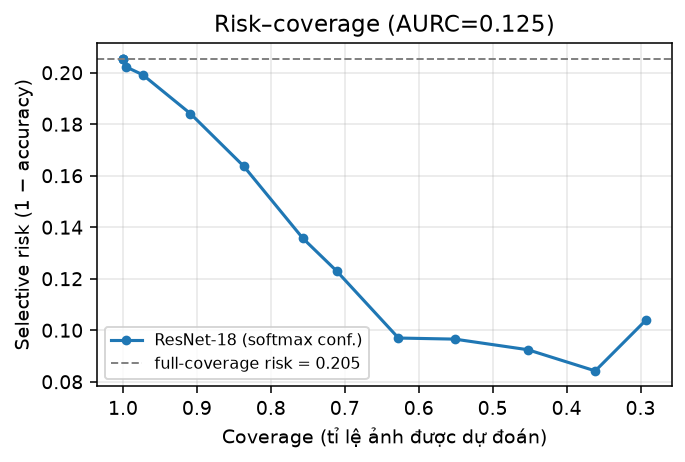
\includegraphics[width=0.72\textwidth]{figures/selective_prediction.png}
\caption{Selective prediction: selective risk ($1-\text{accuracy}$) versus coverage after temperature scaling. Abstaining on the least-confident cases roughly halves the error rate (AURC $=0.125$).}
\label{fig:riskcoverage}
\end{figure}

\subsection{Stage-Gated Retrieval (RQ2)}

Table~\ref{tab:retrieval} reports the aggregate over all 420 auto-derived scenarios. Adaptive soft gating (P) significantly outperforms the ungated baseline (B0) and the fixed-soft baseline (B3) on nDCG, recall, and stage safety (paired bootstrap, 95\% CI excluding zero). Against the strongest baseline, query expansion (B1), P is statistically tied on nDCG and recall and loses raw precision, but reduces SIRR from 0.159 to 0.039---roughly a threefold reduction in stage-incompatible evidence, the property most relevant to safe advisory retrieval. Hard filtering (B2) achieves the lowest SIRR (0.002) but at a substantial nDCG cost. Figure~\ref{fig:tradeoff} shows the trade-off: P sits near the oracle in the high-nDCG, low-SIRR corner, while B1 attains the best ranking quality at the worst stage safety.

\begin{table}[t]
\centering
\caption{Retrieval over 420 auto-derived scenarios (end-to-end image-based; oracle uses ground-truth stage as an upper bound). Labels are auto-derived from stage-compatibility, not domain-reviewed. Best non-oracle value per column in bold; SIRR lower is better.}
\label{tab:retrieval}
\small
\begin{tabular}{lcccc}
\toprule
\textbf{Method} & \textbf{P@5} & \textbf{R@5} & \textbf{nDCG@5} & \textbf{SIRR@5}$\downarrow$ \\
\midrule
B0: Ungated hybrid & 0.225 & 0.118 & 0.165 & 0.136 \\
B1: Query expansion & \textbf{0.371} & 0.193 & \textbf{0.336} & 0.159 \\
B2: Hard filter & 0.267 & 0.181 & 0.259 & \textbf{0.002} \\
B3: Fixed soft re-ranking & 0.261 & 0.164 & 0.267 & 0.072 \\
P: Adaptive re-ranking & 0.301 & \textbf{0.199} & 0.314 & 0.039 \\
\midrule
Oracle (stage upper bound) & 0.327 & 0.222 & 0.349 & 0.022 \\
\bottomrule
\end{tabular}
\end{table}

Table~\ref{tab:strat} stratifies the same scenarios by whether the image-based prediction is correct, off by one adjacent stage, or off by two or more. On correct (330 scenarios) and adjacent-error (84 scenarios) cases---together $414/420$---adaptive soft gating attains the highest nDCG while keeping SIRR low, confirming that soft gating preserves relevant evidence when the belief is right or close. On the 6 non-adjacent errors the pattern inverts: hard filtering yields the best nDCG and a much lower SIRR (0.100 versus P's 0.333), because when the vision model is confidently wrong by several stages soft gating overweights the incorrect stage. Although $n=6$ is too small for a statistical claim, it shows adaptive gating is not uniformly safer than hard filtering---its advantage is concentrated in the common correct/adjacent regime.

\begin{table}[t]
\centering
\caption{nDCG@5 / SIRR@5 stratified by vision error condition (420 scenarios). Adaptive gating (P) leads on correct and adjacent cases; hard filtering (B2) is safer under rare non-adjacent errors.}
\label{tab:strat}
\small
\begin{tabular}{lccc}
\toprule
\textbf{Method} & \textbf{Correct ($n{=}330$)} & \textbf{Adjacent ($n{=}84$)} & \textbf{Non-adj. ($n{=}6$)} \\
\midrule
B0: Ungated & 0.162 / 0.146 & 0.185 / 0.074 & 0.052 / 0.433 \\
B2: Hard filter & 0.276 / \textbf{0.000} & 0.196 / 0.005 & \textbf{0.184} / \textbf{0.100} \\
B3: Fixed soft & 0.278 / 0.072 & 0.230 / 0.057 & 0.135 / 0.300 \\
P: Adaptive & \textbf{0.334} / 0.034 & \textbf{0.244} / 0.036 & 0.174 / 0.333 \\
\bottomrule
\end{tabular}
\end{table}

\begin{figure}[t]
\centering
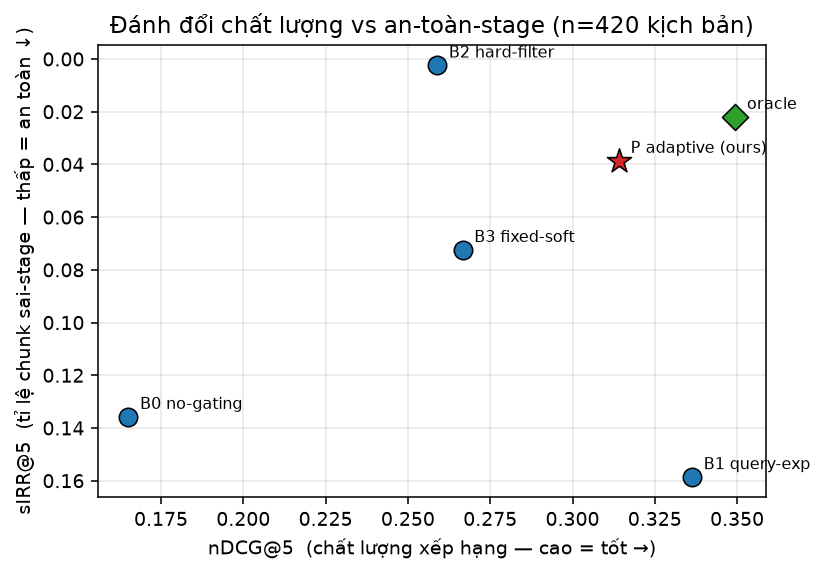
\includegraphics[width=0.72\textwidth]{figures/retrieval_tradeoff.png}
\caption{Ranking quality (nDCG@5, higher better) versus stage safety (SIRR@5, lower better) over 420 scenarios. Adaptive gating (P, star) is near the oracle; query expansion (B1) has the best nDCG but the worst SIRR.}
\label{fig:tradeoff}
\end{figure}

\section{Discussion}

\textbf{RQ1.} On the leakage-audited 2{,}900-image benchmark a fine-tuned ResNet-18 reaches 0.807 accuracy and 0.798 macro-F1, far above the 0.335 majority reference, and the certified-clean splits (Table~\ref{tab:leakage}) mean this is not an artifact of near-duplicate memorization. The more interesting finding concerns the objective: overall accuracy and MASD do not distinguish the three losses beyond seed noise, so the ordinal loss's genuine contribution is not higher accuracy but the \emph{stability} of reproductive-stage recall. For a safety-critical, data-scarce stage, a model that behaves identically across reruns is preferable to one that is on average similar but volatile. We do not overclaim: the mean reproductive-recall difference is not significant even pooled ($n=72$, $p=0.29$), so ``stable'' is the claim, not ``higher.''

\textbf{RQ2.} Confidence-aware soft gating is more robust than hard filtering for the common case, with an honest boundary. It significantly beats the ungated and fixed-soft baselines everywhere and matches the strongest baseline on ranking quality while cutting stage-incompatible retrievals threefold. Crucially, the stratified view shows this is not a uniform win: soft gating leads when the belief is correct or off by one adjacent stage ($414/420$ cases), but under rare non-adjacent errors a calibrated model can be confidently wrong and hard filtering is safer. This is exactly the trade-off the method is designed around, and it argues for pairing soft gating with the abstention policy of Fig.~\ref{fig:riskcoverage} so that low-confidence, likely-severe-error cases are routed to a human.

\textbf{RQ3.} Errors concentrate in the under-represented stages, and the residual risk the system cannot yet control is the non-adjacent error under high confidence. The retrieval conclusions rest on auto-derived relevance labels, so they establish the pipeline's behavior and metric trends rather than expert-judged effectiveness; the oracle upper bound does achieve the lowest SIRR, indicating the corpus carries usable stage structure.

\section{Limitations and Future Work}
\label{sec:limitations}

Reproductive stage has $n=24$ test images; per-image significance is underpowered (McNemar $p=0.50$, and $p=0.29$ even when the three seeds are pooled to $n=72$), so we frame the ordinal loss's benefit as recall stability across seeds ($\sigma=0$ versus $0.071$) rather than a significant single-run gain. Retrieval relevance is auto-derived from stage-compatibility, not expert-annotated, so the retrieval tables are a preliminary automated evaluation; a domain-reviewed relevance set would also let us report pure oracle-stage retrieval for every method. The temporal-prior fusion in the method is exercised only on simulated monotonic trajectories and is not part of the reported results. Focal loss degraded calibration and is included only as a negative ablation. Finally, the perceptual-hash audit certifies the benchmark is free of near-duplicate leakage, but it is complementary to field- or season-grouped splitting, which cannot yet be exercised because RiceSEG carries no field/session identifiers; recovering that metadata, and coupling soft gating with abstention on non-adjacent-error risk, are the priority next steps.

\section{Ethical Considerations}

Farm images can reveal location, farm layout, or other information the grower may not want disclosed, so any public release should strip personal identifiers and precise geolocation unless the source has explicitly consented. The system is a research component feeding a larger decision-support pipeline, not an autonomous authority on agronomic decisions. Outputs involving pesticides, dosage, withholding periods, or regulated actions must be grounded in current authoritative sources, and low-confidence predictions should prompt a request for a better image or an uncertainty flag rather than a definitive-sounding recommendation.

\section{Conclusion}

CropState-Vision recognizes six BBCH-derived rice growth stages from field images and uses the full stage distribution to gate evidence retrieval. On a 2{,}900-image benchmark whose splits are certified free of near-duplicate leakage, a fixed-split, multi-seed study shows a fine-tuned ResNet-18 reaches 0.807 accuracy, and among training objectives an ordinal-aware loss stabilizes reproductive-stage recall without changing accuracy while a focal loss degrades calibration. Casting confidence as selective prediction halves the error rate when the model abstains on its least-confident cases. On a preliminary evaluation over 420 auto-derived scenarios, adaptive soft gating matches the strongest baseline in ranking quality while cutting stage-incompatible retrievals about threefold, with a clearly bounded exception under rare non-adjacent errors. Two honesty caveats govern these claims: the reproductive-recall advantage is a stability result rather than a significant increase at this sample size, and the retrieval labels are auto-derived rather than domain-reviewed. A domain-reviewed relevance set and field- or season-grouped metadata are the two items that would convert these findings into deployment-grade evidence.

\bibliographystyle{splncs04}
\bibliography{references}

\end{document}
